\documentclass[11 pt]{article}
\usepackage{graphicx}
\usepackage[export]{adjustbox}
\usepackage{float}
\usepackage{amsmath}
\usepackage{pgfplots}
\pgfplotsset{compat=1.15}
\title{EE312 Take-Home Exam 3}
\date{2018\\ March}
\author{Nail Tosun - 2094563 \\ Electric and Electronic Engineering Departmant, METU}
\begin{document}
\maketitle
1)
\subsection*{Saturation only enhancement load}
\begin{figure}[H]
\centering
  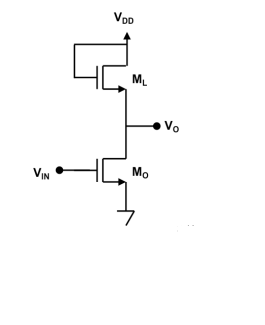
\includegraphics[scale=0.7]{saturationonly}
  \caption{Saturation only enhancement load}
  \label{fig:zero}
\end{figure}
\subsubsection*{Output high calculation}
Since $M_L$ is always in saturation;
\[V_{DS}>V_{GS}-V_{TN} \>\>\> V_D=V_G\]
\[I_{DS}=K_L(\frac{ V_{GS}-V_{TN})^2}{2}=0\]
\[V_{GS}=V_{TN} \>\>\> V_G=V_{DD}\]
\[V_S=V_{OUT}=V_{DD}-V_{TN}=5-0.8=4.2 \> V\]
\subsubsection*{Input low calculation}
After $M_O$ open since both transistor in saturation region;
\[I_{DS}=\frac{K_O(V_{in}-V_{TH})^2}{2} =\frac{K_L(V_{DD}-V_{out}-V_{TH})^2}{2}\]
by mean before $M_L$ goes into linear region $V_{out}$ is linearly change with $V_{in}$. Therefore we have to choose conservative input low voltage;
\[V_{IL}=V_{TH}=0.8 \>V\]

\subsubsection*{Output low calculation}
To find output low voltage first assume after some point $M_L$ is go into linear region since $V_{DS}$ is sufficiently dropped. Keep in mind $M_L$ is always in saturation region.
\[I_{DS}=\frac{K_O(V_{DD}-V_{TH}-V_{out})^2}{2}=K_N(V_{in}-V_{TH})(V_{out})-\frac{K_N V_{out}^2}{2}\]
\[V_{in}=4.2 V\]
Put $V_{in}=4.2V$ and solve for $V_{out}$
\[V_{OL}=1.12\> V\]
\subsubsection*{Input high calculation}
To find input high calculation we should find $\frac{dV_{out}}{V_{in}}=-1$ point.
\[I_{DS}=\frac{K_O(V_{DD}-V_{TH}-V_{out})^2}{2}=K_N(V_{in}-V_{TH})(V_{out})-\frac{K_N V_{out}^2}{2}\]
Taking derivative both side with $\frac{d}{dV_{in}}$;


\subsubsection*{Critical Voltage}
The voltage with when $M_0$ goes into linear region.
\[V_{DS}=V_{GS}-V_{TN}\]
\[V_{out}=V_{in}-0.8 \tag{1} \label{eq:1} \] 
\[I_{DS}=\frac{K_O(V_{GS}-V_{TN})^2}{2}=\frac{K_N(V_{DD}-V_{TH}-V_{out})^2}{2}\]
\[\sqrt{\frac{3}{2}}(V_{in}-0.8)=4.2-V_{out}\tag{2} \label{eq:2} \]
Putting \eqref{eq:1} and \eqref{eq:2} together;
\[V_{in}=2.69 V\]
\[V_{critical}=1.89 V\]
\subsubsection*{Voltage Transfer Characteristic}

\subsection*{Resistive loaded NMOS}
First ($V_{in}=0$) NMOS is in cut-off region. When $V_{in}$ pass the threshold voltage it is go into saturation region since large $V_{DS}$ then eventually it goes into linear region.
\subsubsection*{Input low voltage}
\[I_{DS}=\frac{K_N(V_{GS}-V_{TH})^2}{2}=\frac{V_{DD}-V_{out}}{R_L}\]
To be able to find input low voltage we should look at $\frac{dV_{out}}{dV_{in}}=-1$;
\[\frac{(V_{in}-0.8)^2}{2}=\frac{5-V_{out}}{K_NR_L}\]
\[V_{in}-0.8=-0.44\frac{dV_{out}}{dV_{in}}\]
\[V_{IL}=1.24 \>V\]
\subsubsection*{Output high voltage}
Since NMOS is in cut-off when input low and output high $V_{OH}=5 \>V$
\subsubsection*{Input high voltage}
Since both expression for current is true;
\[(V_{in}-V_{TN})V_{out}-\frac{V_{out}^2}{2}=\frac{V_{DD}-V_{out}}{R_L K_n} \tag{3} \label{eq:3} \]
Taking derivative of both side with $\frac{d}{dV_{in}}$;
\[
2V_{out}-V_{in}+0.8=0.44 \tag{4} \label{eq:4}
\]
Putting \eqref{eq:3} and \eqref{eq:4} in same equation and solve for $V_{in}$;
\[V_{IH}=2.78\>V\]
\subsubsection*{Output low voltage}
\[I_{DS}=K_N((V_{GS}-V_{TN})V_{out}-\frac{V_{out}^2}{2})\]
\[I_{DS}=K_N(4.2V_{out}-\frac{V_{out}^2}{2})=\frac{5-V_{out}}{R_L}\]
\[(4.2V_{out}-\frac{V_{out}^2}{2})=\frac{5-V_{out}}{K_NR_L}\]
\[(4.2V_{out}-\frac{V_{out}^2}{2})=0.44(5-V_{out})\]
Solving quadratic equation;
\[V_{OL}=0.50\>V\]
\subsection*{Depletion mode NMOS load}
Firstly, when $V_{in}=0V$ $M_O$ is cut-off and $M_D$ is in linear region since there is no $I_{DS}$ current.
\subsubsection*{Input low voltage}
\[I_{DS}=\frac{K_O(V_{GS}-V_{TH})^2}{2}=K_D((V_{GS}-V_{TH})V_{DS}-\frac{V_{DS}^2}{2})\]
\[I_{DS}=\frac{K_O(V_{in}-0.8)^2}{2}=K_D((-V_{TH})(V_{DD}-V_{out})-\frac{(V_{DD}-V_{out})^2}{2})\]
Taking derivative two side with $\frac{d}{V_{in}}$
\[V_{in}-0.8=-0.8\frac{dV_{out}}{dV_{in}}+\frac{dV_{out}(5-V_{out})}{dV_{in}}\]
Then putting $\frac{dV_{out}}{dV_{in}}=-1$
\[V_{out}=3.4+V_{in}\]
Putting above equation into current equation and solve for $V_{in}$ 
\[V_{in}=1.37 \> V\]
\subsubsection*{Input high voltage}
Then $M_D$ is in saturation region whereas $M_O$ linear region 
\[I_{DS}=\frac{K_D(V_{GS}-V_{TH})^2}{2}=K_O((V_{in}-0.8)V_{DS}-\frac{V_{DS}^2}{2})\]
\[0.32=(V_{in}-0.8)V_{DS}-\frac{V_{DS}^2}{2}\]
\[0.32=(V_{in}-0.8)V_{out}-\frac{V_{out}^2}{2}\]
Taking derivative two side with $\frac{d}{V_{in}}$
\[V_{in}-0.8=2V_{out}\]
Putting above equation into current equation and solve for $V_{in}$
\[V_{IH}=1.72 \>V\]

\subsubsection*{Output low voltage}
To find $V_{out}$ we should give input as 5V to the input high case current equation(where $M_D$ is in saturation region $M_O$ linear region ).
\[V_{OL}=0.08 \>V\]

\subsubsection*{Output high voltage}
Since we used depletion mode NMOS transistor in pull-up network ($V_{TN}$<0) $V_{out}=V_{DD}=5\> V$
\subsection*{Conclusion}
\subsubsection*{Voltage Swings}
Only with depletion load NMOS inverter we can achieve rail-tp-rail operation. With saturation only load NMOS inverter since up transistor in saturation region $V_{GS}>V_{TN}$
(with positive threshold voltages) $V_S=V_{out}$ always less than $V_{DD}$. Moreover with resistive NMOS inverter although we have $V_DD$ at output high still we have nonzero output low and we have significant static power consumption. If we order voltage swings numerically;
$$VS_{depletion}>VS_{resistive}>VS_{saturation-only}$$
\subsubsection*{Noise Margins}
Depletion NMOS load case:

NMH=$V_{OH}-V_{IH}=3.28 \> V $

NML=$V_{IL}-V_{OL}=1.29\> V $

Saturated-only NMOS load case:

NMH=$V_{OH}-V_{IH}= 1.42 \>V$

NML=$V_{IL}-V_{OL}= -0.32$

Since $V_{IL}$ can't be smaller than output low voltage this inverter don't work properly.

Resistive only NMOS load case:

NMH=$V_{OH}-V_{IH}= 2.21 \>V$

NML=$V_{IL}-V_{OL}= 0.31 \>V$

2)
\begin{figure}[H]
\centering
  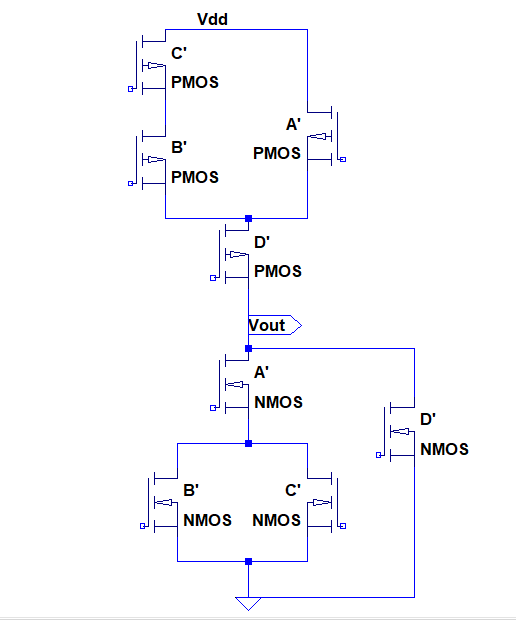
\includegraphics[scale=0.7]{cmos}
  \caption{CMOS design}
  \label{fig:zero}
\end{figure}
\begin{figure}[H]
\centering
  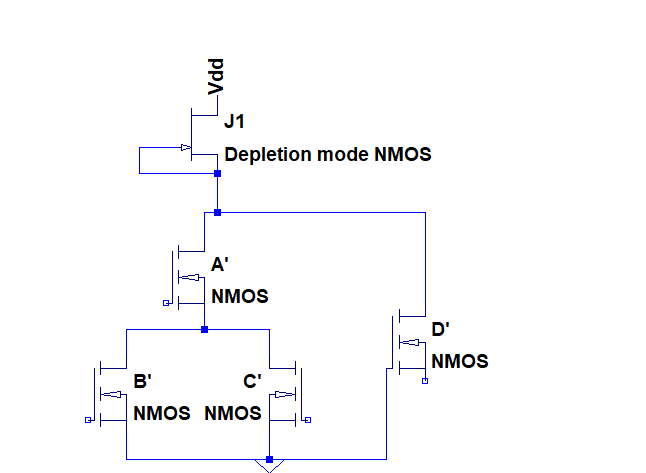
\includegraphics[scale=0.7]{depletion}
  \caption{NMOS depletion loaded design}
  \label{fig:zero}
\end{figure}
\end{document}